% -*- TeX:UK -*-
\documentclass[10pt]{beamer}
\usetheme{metropolis}
%\useinnertheme{rectangles}
\setbeamercovered{%
still covered={\opaqueness<1->{15}},
again covered={\opaqueness<1->{40}}}

\hypersetup{colorlinks,linkcolor=black,urlcolor=brown,citecolor=brown}

\usepackage{amsmath,amssymb,amsthm}
\usepackage{unicode-math}

% We set the Lucida OTF fonts as default
\usepackage{fontspec}
\setmainfont{Lucida Bright OT}
\setsansfont{Lucida Sans OT}
\setmonofont{Lucida Console DK}[Scale=MatchLowercase]

\newfontfamily\webglyphsfont{WebHostingHub-Glyphs}[Scale=0.7]
\newcommand\webglyphs[1]{{\webglyphsfont\symbol{#1}}}
\newcommand\Discussion{\colorbox{white}{\textcolor{black}{\webglyphs{"F134}}}\xspace}
\newcommand\DiscussionI{\colorbox{black}{\textcolor{white}{\webglyphs{"F134}}}\xspace}
\newcommand\DExamples{\colorbox{black}{\textcolor{white}{\webglyphs{"F134} examples?}}}
\newcommand\Reading{\colorbox{black}{\textcolor{white}{\webglyphs{"F0C1}}}\xspace}
\newcommand\ReadingI{\colorbox{white}{\textcolor{black}{\webglyphs{"F0C1}}}\xspace}
\newcommand\Video{\colorbox{white}{\textcolor{black}{\webglyphs{"F03D}}}\xspace}
\newcommand\Attention{\colorbox{black}{\textcolor{orange}{\webglyphs{"F05A}}}\xspace}
\newcommand\HomeWork{\colorbox{white}{\textcolor{black}{\webglyphs{"F5ED}}}\xspace}
\newcommand\HomeWorkI{\colorbox{black}{\textcolor{white}{\webglyphs{"F5ED}}}\xspace}
\newcommand\Advanced{\colorbox{black}{\textcolor{white}{\webglyphs{"F235}}}\xspace}

\newfontfamily\lineabasicfont{linea-basic-10}
\newcommand\basicicons[1]{{\lineabasicfont\symbol{#1}}}
\newcommand\timeforwards{\basicicons{"0079}}
\newcommand\timebackwards{\basicicons{"0064}}

\newfontfamily\lineaweatherfont{linea-weather-10}
\newcommand\weathericons[1]{{\lineaweatherfont\symbol{#1}}}
\newcommand\meteosun{\weathericons{"E038}}
\newcommand\meteosuncloud{\weathericons{"E042}}
\newcommand\meteorain{\weathericons{"E033}}
\newcommand\meteowind{\weathericons{"E054}}

\newfontfamily\uleaffont{Mini Pics Uprooted Leaf}
\newcommand\uleafmpics[1]{{\uleaffont\symbol{#1}}}
\newcommand\lowplants{\uleafmpics{"00CE}}
\newcommand\mediumplant{\uleafmpics{"006A}}
\newcommand\bush{\uleafmpics{"0039}}
\newcommand\smallplant{\uleafmpics{"0030}}
\newcommand\seedling{\uleafmpics{"002F}}
\newcommand\floweringplant{\uleafmpics{"00CA}}

\newfontfamily\utwigfont{Mini Pics Uprooted Twig}
\newcommand\utwigmpics[1]{{\utwigfont\symbol{#1}}}
\newcommand\grassplant{\utwigmpics{"0033}}

\newfontfamily\uinsectfont{Insect Icons}
\newcommand\uinsect[1]{{\uinsectfont\symbol{#1}}}
\newcommand\bug{\uinsect{"006F}}

\usepackage{polyglossia}
\setdefaultlanguage[variant = british, ordinalmonthday = false]{english}

\usepackage[style=authoryear-comp,firstinits,sortcites,maxcitenames=2,%
    mincitenames=1,maxbibnames=10,minbibnames=10,uniquename=mininit,%
    uniquelist=minyear,sortfirstinits=true]{biblatex}
\addbibresource{../references/ecophys.bib}
\renewcommand{\bibfont}{\small}

\usepackage{abbrev}



\usepackage{tikz}
\usetikzlibrary{positioning,fit,arrows}

\tikzset{
 big dot/.style
  = {circle, draw, inner sep=0pt, minimum size=3mm, fill=teal!50},
 a/.style
  = {node distance=4em, text width=0.1em, minimum height=4em},
 b/.style
  = {rectangle, draw, fill=gray!10, node distance=4em, text width=6em,
     text centered, rounded corners, minimum height=4em, thick},
 c/.style
  = {circle, draw, dashed, fill=orange!10, inner sep = 0pt, node distance=5em, text width=6em,
     text centered, thick},
 d/.style
  = {rectangle, draw, dashed, fill=red!10, node distance=4em, text width=6em,
     text centered, rounded corners, minimum height=4em, thick},
 l/.style
  = {draw, -latex, ultra thick},
 lr/.style
  = {draw, latex-latex, ultra thick, red},
 lb/.style
  = {draw, -latex, ultra thick, blue},
  lo/.style
  = {draw, -latex, ultra thick, orange},
  lg/.style
  = {draw, -latex, ultra thick, teal},
  mylabel/.style
  ={text width=6.5em, text centered},
 aa/.style
  = {node distance=4em, text width=0em, minimum height=0.5ex},
 ll/.style
  = {draw, {open triangle 45} -, thick},
 llb/.style
  = {draw, - triangle 45, thick, blue},
 llg/.style
  = {draw, - open triangle 45, thick, green},
  llt/.style
  = {draw, - open triangle 45, thick, teal},
 llr/.style
  = {draw, - triangle 45, thick, purple},
 llo/.style
  = {draw, - triangle 45, thick, orange}
}


\begin{document}

\title{PBIO-141\\Sensory and Physiological Ecology\\of  Plants}
\subtitle{2: Terminology and viewpoint}
\author{Pedro J. Aphalo}
\date{January--February 2022}
\institute[Univ.\ of Helsinki]{M.Sc.\ in Plant Biology, University of Helsinki\\[2ex] \url{http://blogs.helsinki.fi/aphalo/}\\[2ex] \url{mailto:pedro.aphalo@helsinki.fi}}

\begin{frame}
\maketitle
\end{frame}

  \begin{frame}[c]
    \begin{center}
      \begin{small}
        \copyright 2006--2022 by Pedro J. Aphalo\\
        University of Helsinki, Finland.\\
        \textcolor{blue}{\url{http://blogs.helsinki.fi/senpep-blog/}}\\[2ex]
      \end{small}

      \begin{footnotesize}
        Sensory and Physiological Ecology of Plants slides by Pedro J. Aphalo are licensed under a Creative Commons Attribution-ShareAlike 4.0 International License.

      
\includegraphics[width=6em]{../figures/copyright/by-sa}\\[2ex]
      \end{footnotesize}
        
        \begin{scriptsize}
        Typeset in Lucida Sans, \textrm{Luicda Bright}, \texttt{Lucida Console} and Lucida Math. Icons from fonts ``WebHostingHub Glyphs'' (under SIL-Open Font License) from \url{https://www.webhostinghub.com/}; ``insect icons'' (free from \url{http://www.woodcutter.es/}); ``linea-basic-10'' and ``linea-weather-10'' (free from \url{https://github.com/linea-io}), ``Mini Pics Uprooted Twig'' and ``Mini Pics Uprooted Twig'' (commercial, from Image Club Graphics, Inc.). Plant icon as .svg by Abdul Wahhab (free from \url{NounProject.com}).

        Illustrations and text quoted from copyrighted sources is excluded from this license and their use should respect the original licenses.
        \end{scriptsize}
    \end{center}
  \end{frame}


\begin{frame}
    \frametitle{Outline}
    \tableofcontents
\end{frame}

\section{Adaptation vs.\ acclimation}

\begin{frame}{\HomeWork Wild plants vs.\ weeds vs.\ crops \Discussion 10 + 5 min}
    \begin{itemize}

        \item<1,4> Most \textbf{crops} have been under artificial selection for a
        long time. Farmers and breeders have selected the most useful
        genotypes.

        \item[{\small +}]<1,4> In addition natural selection is also active on cultivated plants,
        although in a managed environment. \DExamples

        \item[{\small --}]<1,4> Most crops have very low fitness in the wild. \DExamples

        \item<2,4> Crop \textbf{weeds} are not subject to artificial selection,
        they are under natural selection but in a managed environment. \DExamples

        \item<3,4> Natural selection in most populations of \textbf{wild plants} is affected by human activities. \DExamples
    \end{itemize}
\end{frame}

\begin{frame}{Adaptation vs.\ acclimation}
\nocite{Aphalo2021a}
\begin{description}
\item[Adaptation] Genetic variation + natural selection. It takes place
over more than one generation. \textit{There is change in the
genotype}.

\item[Acclimation] Regulation within the lifetime of an individual, it
involves changes in the phenotype in response to the environment.
\textit{There is no change in the genotype}.
\end{description}

\footnotesize
\resizebox{\linewidth}{!}{%
  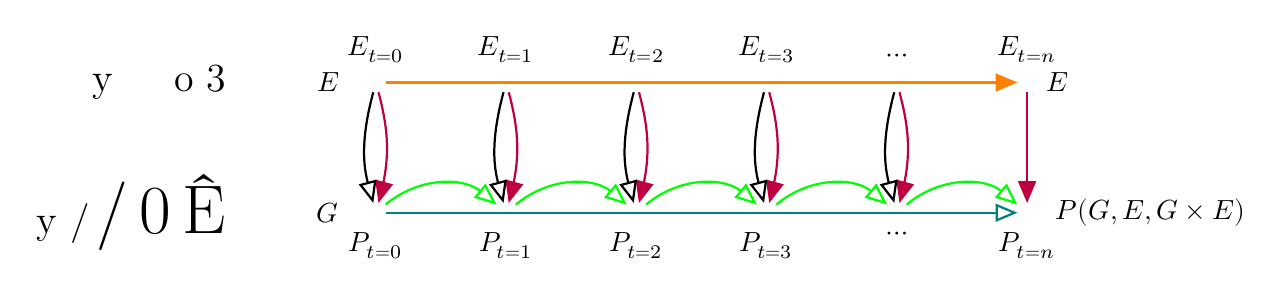
\begin{tikzpicture}[auto]
    \node [aa, label=left:{\Large\timeforwards~\meteosuncloud~\meteorain~\bug~\grassplant}] (environment) {};
    \node [aa, below = of environment, label=left:{\Large\timeforwards~\seedling\,\Huge\seedling\,\smallplant\,\floweringplant}] (plant) {};
    \node [aa, right = of environment, label=above:{$E_{t=0}$}, label=left:{$E\ \ $}] (env_zero) {};
    \node [aa, right = of env_zero, label=above:{$E_{t=1}$}] (env_one) {};
    \node [aa, right = of env_one, label=above:{$E_{t=2}$}] (env_two) {};
    \node [aa, right = of env_two, label=above:{$E_{t=3}$}] (env_three) {};
    \node [aa, right = of env_three, label=above:{$\cdots$}] (env_four) {};
    \node [aa, right = of env_four, label=above:{$E_{t=n}$}, label=right:{$E$}] (env_end) {};
    \node [aa, below = of env_zero, label=below:{$P_{t=0}$}, label=left:{$G\ \ $}] (pheno_zero) {};
    \node [aa, below = of env_one, label=below:{$P_{t=1}$}] (pheno_one) {};
    \node [aa, below = of env_two, label=below:{$P_{t=2}$}] (pheno_two) {};
    \node [aa, below = of env_three, label=below:{$P_{t=3}$}] (pheno_three) {};
    \node [aa, below = of env_four, label=below:{$\cdots$}] (pheno_four) {};
    \node [aa, below = of env_end, label=below:{$P_{t=n}$}, label=right:{\ $P(G, E, G \times E)$}] (pheno_end) {};

    \path [llo, below] (env_zero) -- (env_end);
    \path [llt, above] (pheno_zero) -- (pheno_end);

    \path [llr] (env_zero) edge [bend right=-15] (pheno_zero);
    \path [ll] (pheno_zero) edge [bend right=-15] (env_zero);
    \path [llg, above] (pheno_zero) edge [bend right=-40] (pheno_one);

    \path [llr] (env_one) edge [bend right=-15] (pheno_one);
    \path [ll] (pheno_one) edge [bend right=-15] (env_one);
    \path [llg, above] (pheno_one) edge [bend right=-40] (pheno_two);

    \path [llr] (env_two) edge [bend right=-15] (pheno_two);
    \path [ll] (pheno_two) edge [bend right=-15] (env_two);
    \path [llg, above] (pheno_two) edge [bend right=-40] (pheno_three);

    \path [llr] (env_three) edge [bend right=-15] (pheno_three);
    \path [ll] (pheno_three) edge [bend right=-15] (env_three);
    \path [llg, above] (pheno_three) edge [bend right=-40] (pheno_four);

    \path [llr] (env_four) edge [bend right=-15] (pheno_four);
    \path [ll] (pheno_four) edge [bend right=-15] (env_four);
    \path [llg, above] (pheno_four) edge [bend right=-40] (pheno_end);

    \path [llr] (env_end) -- (pheno_end);

  \end{tikzpicture}%
}%

\textrm{\textbf{Figure:} Time course of one realization of the environment ($E$) during the lifetime of an individual of a genotype ($G$) resulting in a phenotype ($P$).}
\end{frame}

\begin{frame}{Adaptation vs.\ acclimation \Discussion 5 min}

\textbf{Examples of adaptation}

Shade $\rightarrow$ larger and thinner leaves.\\
Drought $\rightarrow$ larger root:shoot weight ratio.\\
Hot + dry environment $\rightarrow$ CAM photosynthesis.\\[2ex]

\textbf{Examples of acclimation}

Shade $\rightarrow$ larger and thinner leaves.\\
Drought $\rightarrow$ larger root:shoot weight ratio.\\
Hot + dry environment $\rightarrow$ CAM photosynthesis.\\[2ex]
\pause

\DiscussionI \emph{How is it possible that the examples can be the same? Where is the difference?}

\end{frame}

\begin{frame}{You are a seed in the soil \Discussion 10 + 10 min}

Discuss this topic in groups of 2 or 3 students (10 min). Take notes while discussing and have them ready for general discussion (10 min).

\begin{alertblock}{Thought exercise: when should I germinate?}
\begin{enumerate}
  \item Write a list of dangers you are exposed to.
  \item Write a list of good opportunities you have.
  \item Write a list of conditions you can perceive around you.
  \item What information can you obtain?
  \item How would you use this information to decide to germinate of not?
\end{enumerate}
\end{alertblock}

\end{frame}

\section{Plants and animals}

\begin{frame}{Plants $\neq$ animals}

\center
\begin{tabular}{lll}
\hline
& \textbf{Plants} & \textbf{Animals}\\
\hline
Mobility & sessile & mobile\\
Structure & modular & fixed\\
Growth & indeterminate & determinate\\
Energy source & light & organic substances\\
Nervous system & no & yes\\
\hline
\end{tabular}
%\vspace{5mm}
\end{frame}

\begin{frame}{Plants $\approx$ animals}

\center
\begin{tabular}{lll}
\hline
& \textbf{Plants} & \textbf{Animals}\\
\hline
Structure & complex & complex\\
Function & complex  & complex\\
Behaviour & complex & complex\\
Sensing & yes & yes\\
Communication & `yes' & yes\\
Memory & `yes' & yes\\
Problem solving & `yes' & yes\\
Learning & `yes' & yes\\
\hline
\end{tabular}
\end{frame}

\begin{frame}{Challenges of plant research + \Discussion}

\begin{itemize}
    \item<1-2> We need to recognize very different ways of behaving, communicating, and perceiving compared to our own.
    \item<1-2> We should avoid projecting our own human image on the behaviour we observe in plants.
    \item<1-2> We should analyse characteristics and behaviour in relation to life history and fitness.
\end{itemize}

\begin{alertblock}<2>{Plants' `senses' \DiscussionI 5 + 5 min}
  \vspace{0.5ex}
  What features of their environment can plants perceive?\\
\end{alertblock}

\end{frame}

\section{General system theory}
\nocite{Meadows2008,Jones2015}

\begin{frame}{Basic concepts}
  \begin{itemize}
    \item Similar structures and properties are present in all systems.
    \item Possible behaviour is determined by the structure of a ``whole thing''.
    \item The structure emerges from the interactions among its ``component parts''.
    \item If interactions exist, then the contribution of the parts to the behaviour of the ``whole'' depends on the nature of interactions.
    \item Behaviour of a complex whole cannot be predicted from the behaviour of the parts.
    \item ``Emergent properties'' appear as a result of the interactions.
  \end{itemize}
\end{frame}

\begin{frame}{Basic concepts}
  \begin{itemize}
    \item Systems can be nested in other systems.
    \item Thus a hierarchy appears.
    \item A crucial concept is feedback, which can be positive or negative.
    \item \emph{Thinking in systems} is applicable to engineering, computing, human society, business administration, biology, ecology, medicine, etc.
    \item Even to managing everyday life by an individual.
    \item At its simplest, \emph{Thinking in systems} .can be defined as being aware of the ``big picture''.
  \end{itemize}
\end{frame}

\section{Hierarchy and scale}
\nocite{Allen1982}
\begin{frame}{What is hierarchy? \Discussion 5 + 5 min}
  \begin{alertblock}{Hierarchies in biology \Discussion}
    \begin{itemize}
      \item Think examples of the application of the concept of \emph{hierarchy} in biology.
    \end{itemize}
  \end{alertblock}
\end{frame}

\begin{frame}{Hierarchy I}

The term \textit{hierarchy} is frequently used in an intuitive way,
but Allen and Starr (1982) have developed a theory, mainly focused
on ecological systems.

\begin{quotation}
By \textit{hierarchy} we understand a system of behaviour
relationships where upper levels limit and control the lower levels
in a greater or smaller measure depending on the \textbf{time
constants} of their behaviour.
\end{quotation}

\end{frame}

\begin{frame}{Hierarchy II}
\begin{itemize}
\item Where \textit{time constant} of a response is the length of time
between when a response to a stimulus starts to be observable until
it reaches a certain level close to the maximum that the given
stimulus will induce. It is a measure of the speed of change of a
response to an instantaneous stimulus.

\item In contrast \textit{lag} is the delay between the application of
the stimulus and the start of an observable response.
\end{itemize}
\end{frame}

\begin{frame}{Hierarchy III}

The degree of control, that is the asymmetry of the relationship,
depends on the time constants of the behaviour.

\vspace{\stretch{1}} \center{\fbox{\parbox{0.8\textwidth}{When we
study the mechanism of a system at one level, we can ignore what changes much more slowly
(has a larger time constant).}}} \vspace{\stretch{1}}

\vspace{\stretch{1}} \DExamples\vspace{\stretch{1}}

\end{frame}

\begin{frame}{Hierarchy IV: examples}
\begin{itemize}
\item For example if we study the evolution of plants on Earth we can
ignore the big bang and the expansion of the universe (and many
other things).

\item If we are interested \emph{only} (narrowly?) in the response of photosynthesis to light
in Arabidopsis, we can ignore the evolution of plant species.

\item If we are interested only in the primary reactions of photosynthesis
we can use in our experiments isolated chloroplasts and ignore the
plant.
\end{itemize}
\end{frame}

\section*{References}
\nocite{Chamovitz2017,Denison2012,Karban2015,Keddy2017,Manetas2012}
\nocite{Sadras2021,Sadras2014a}
  \begin{frame}[t,allowframebreaks]
    \frametitle{References}
    \printbibliography
  \end{frame}

\end{document}

